\documentclass[12pt, notitlepage, final]{article}

\newcommand{\name}{Vince Coghlan and Zach Vogel}

%\usepackage[dvips]{graphics,color}
\usepackage{amsfonts}
\usepackage{amssymb}
\usepackage{amsmath}
\usepackage{latexsym}
\usepackage{enumerate}
\usepackage{amsthm}
\usepackage{nccmath}
\usepackage{setspace}
\usepackage[pdftex]{graphicx}
\usepackage{epstopdf}
\usepackage[siunitx]{circuitikz}
\usepackage{tikz}
\usepackage{float}
\usepackage{cancel}
\usepackage{setspace}
\usepackage{overpic}
\usepackage{mathtools}
\usepackage{listings}
\usepackage{color}
\usepackage{qtree}
\usepackage{pgfplots}
\usepackage{pdflscape}
%\usepackage{gensymb}

\usetikzlibrary{calc}
\usetikzlibrary{matrix}
\usetikzlibrary{positioning}

%\numberwithin{equation}{section}
\newcommand{\dbr}[1]{d_{\mbox{#1BR}}}
\newtheorem{lemma}{Lemma}
\newtheorem*{corollary}{Corollary}
\newtheorem{theorem}{Theorem}
\newtheorem{proposition}{Proposition}
\theoremstyle{definition}
\newtheorem{define}{Definition}

\newdimen\digitwidth{}
\settowidth\digitwidth{0}
\def~{\hspace{\digitwidth}}

\setlength{\parskip}{1pc}
\setlength{\parindent}{0pt}
\setlength{\topmargin}{-3pc}
\setlength{\textheight}{9.0in}
\setlength{\oddsidemargin}{0pc}
\setlength{\evensidemargin}{0pc}
\setlength{\textwidth}{6.5in}

\DeclareMathOperator*{\argmin}{arg\,min}

%absolute value code
\DeclarePairedDelimiter\abs{\lvert}{\rvert}%
\DeclarePairedDelimiter\norm{\lVert}{\rVert}
\makeatletter
\let\oldabs\abs{}
\def\abs{\@ifstar{\oldabs}{\oldabs*}}
%
\let\oldnorm\norm{}
\def\norm{\@ifstar{\oldnorm}{\oldnorm*}}
\makeatother

\def\dbar{{\mathchar'26\mkern-12mu d}}
%\def \P[x]{\Frac{\partial}{\partial x}}
%\def \D[x]{\Frac{d}{dx}}
\newcommand{\PD}[2]{\frac{\partial#1}{\partial#2}}
\newcommand{\PF}[1]{\frac{\partial}{\partial#1}}
\newcommand{\DD}[2]{\frac{d#1}{d#2}}
\newcommand{\DF}[1]{\frac{d}{d#1}}
\newcommand{\fix}[2]{\left(#1\right)_#2}
\newcommand{\ket}[1]{|#1\rangle}
\newcommand{\bra}[1]{\langle#1|}
\newcommand{\braket}[2]{\langle{} #1 | #2 \rangle}
\newcommand{\bopk}[3]{\langle{} #1 | #2 | #3 \rangle}
\newcommand{\Choose}[2]{\displaystyle{} {#1 \choose{} #2}}
\newcommand{\proj}[1]{\ket{#1}\bra{#1}}
\def\del{\vec{\nabla}}
\newcommand{\avg}[1]{\langle#1\rangle}
\newcommand{\piecewise}[4]{\left\{\beginProtected{array}{rl}#1&:#2\\#3&:#4\endProtected{array}\right.}
\newcommand{\systeme}[2]{\left\{\beginProtected{array}{rl}#1\\#2\endProtected{array}\right.}
\def\Godel{G$\ddot{\mbox{o}}$del}

\title{Cache Simulator}
\date{\today}
\author{\name}

\begin{document}

\maketitle


\section{Introduction}

Cache configurations are not a one size fits all job.  Some cache's are better than others for specific
applications.  For example, a multiway cache will benifit a system that has limited space, as hit rates
will increase.  A direct-mapped cache will be better for a larger cache, since our hit times will be very
fast.  Our simulations are an attempt to discover some of these facts.  We created a simulator that will
preform instruction, read, and write operations on any associativity or size cache.  This cache system
included a hierarchy of a level 1 instruction cache, a level 1 data cache, and a unified level two cache.
The caches are all write-allocate, write-back, meaning writes will immidiately write to the cache, and any
data in the cache that has been written must be accounted for and lazily written back down to level two and
eventually main memory.  All caches maintain their own Least Recently Used (LRU) policy in order to preform
the best that they can given information at any point in execution.  We measured many metrics, such as hit
time, miss time, cost, CPI, ideal times, and kickouts.  Although many things are idealized, this simulator
is very similar to what you would see in a modern computing machine.

\section{Design}
There were several design considerations of note that must be addressed.  The first concern of ours, was one
of memory.  The stack was stored as an array of structures in heap memory.  This was mainly for speed reasons.
An array is generally faster than a linked list when we dont know where in the list we are going.  The second
consideration was how to design the requests.  We found it to be simplist to split the simulator, much like a
computer does, into the CPU portion, and the cache portion.  The CPU decides how many references it needs, and
decides what to do when it gets a hit, miss, or dirty kickout.  The cache portion, on the other hand, was a
simple machine.  It took the address and the cache it was looking in and that is essentially it.  It returned
a hit, miss, or the tag of a dirty kickout that it received.  The CPU simulater then decides what to do with
this information.  The last important consideration was the LRU system.  We knew that the fastest solution
would be to provide each block with a number that would represent it's place in the LRU.  This would be a
constant time solution.  This, however, led to some difficulties in implementation when we had variable sized
caches.  We instead went with a linked list structure.  This made it easy to program, and we knew that for
every cache other than the fully associative, this time would be relatively minimal.

The use of the code is quite simple.  The inluded makefile will build the program on our versions of Mac OSX
10.9 and Arch Linux.  just typing make is sufficient, while make clean will remove the compiled files.  The
libraries used are quite simple.  libc and the POSIX standard library are all that is required.  Once built
the program will be called cachesim.  At that point it can be run with an option describing some features.
cachesim -v will run in "verbose" mode, where each cache reference and clock cycle will be spelled out step
by step.  Besides helping in debugging, it is quite relaxing to watch all the text fly by.  cachesim -h will
print out the usage: "usage: cat $<$traces$>$ $|$ ./cachesim [-hv] $<$config\_file$>$".  Note that the traces
must be sent in through stdin, any other form of stdin will work as well, not just cat.  The config file takes
the form of a series of lines, each with a parameter, followed by a space, then a value.  For example, a line
could be "l1dassoc 4".  That would set the level 1 data cache to a 4-way set associative cache.  A full list
can be seen in the code, or in the example config files provided.

\section{Simulation}
The simulations were run on multiple cores of a PC running Debian Linux virtualized in a windows enviornment.
In total they were run in a little under 20 hours.  The simulations included a number of traces that tested
a variaty of typical operations a computer would run.  Not suprisingly the simulations of the fully
associative caches took almost twice as long as the direct mapped ones.  The LRU's linked list had to be
traversed and reorganized on almost every reference.  This meant slow references, as well as a much less
efficient real-life cache.  We simluated each of the 5 traces on 10 different caches.  Additionally, the
omnetpp simulation was run on systems with multiple memory chunk sizes from cache to main memory.  We will
preform cost benifit analysis on this later.

\section{Results}
\subsection{Cache Configuration}
The best way to present this data, in our minds, is to represent it as a ratio of the real time over the
ideal time.  Since many of the traces vary in ideal execution time, but are mostly proportional to the
stack parameters, the best option to initally analyse the data is to average out the values from each
group of traces and present the ratio over ideal time.  This can be seen below.

\begin{center}
\begin{tikzpicture}
\begin{axis}[
    ybar,
    enlargelimits=0.15,
    title=Execution Time Proportional to Ideal Execution Time,
    ylabel=Ratio Compared to Ideal,
    legend style={at={(0.5,-0.2)},
      anchor=north,legend columns=-1},
    symbolic x coords={default, l1-2way, all-2way, l2-4way, all-4way, l2-big, l1i-small, l1d-small, l1-small, all-FA},
    xtick=data,
    nodes near coords,
	    nodes near coords align={vertical},
    x tick label style={rotate=45,anchor=east},
    width=16cm,
    height=12cm
]
\addplot
coordinates {(default, 17.26) (l1-2way, 15.14) (all-2way, 15.16) (l2-4way, 14.17)
(all-4way, 13.38) (l2-big, 12.62) (l1i-small, 18.14) (l1d-small, 20.52)
(l1-small, 21.53) (all-FA, 12.13)};
\end{axis}
\end{tikzpicture}
\end{center}

The two fastest caches are all-FA and l2-big and, unsuprisingly, the slowest caches are the ones with smaller
l1 cache sizes.  We know that a fully associative cache will gaurantee the highest hit rate.  If we had a very
high miss penalty this would be our best bet, since we would always hit.  The larger L2 cache will also
guarantee a low l2 miss rate which means, less accesses to main memory, the slowest part of the process.

There are reasons why we dont use these caches for our everyday computing.  The fully associative simulation
does not take into account the amount of time it takes to move down the LRU list and update it on every
reference.  It is also extremely expensive, as we will show later on.  The large L2 cache is sufficient to
allow more hits of older data.  This is great, but comes at the cost of a larger cache.

\subsection{Cost}

Cost considerations are very important when considering which cache to choose.  If we manufacture processors,
what matters to us is the bottom line, profit.  The cost multiplied by the preformance as measured above can
give us a good idea of the "best" cache system.

\begin{center}
\begin{tikzpicture}
\begin{axis}[
    ybar,
    enlargelimits=0.15,
    title=Cost Multiplied by Normalized Execution Time,
    scaled y ticks = false,
    yticklabels={,,},
    legend style={at={(0.5,-0.2)},
      anchor=north,legend columns=-1},
    symbolic x coords={default, l1-2way, all-2way, l2-4way, all-4way, l2-big, l1i-small, l1d-small, l1-small, all-FA},
    xtick=data,
    x tick label style={rotate=45,anchor=east},
    width=16cm,
    height=12cm
]
\addplot
coordinates {(default, 9061.5) (l1-2way, 14004.5) (all-2way, 14781) (l2-4way, 14524.25)
(all-4way, 19066.5) (l2-big, 12304.5) (l1i-small,  7709.5) (l1d-small, 8721)
(l1-small, 6997.25) (all-FA, 50642.75)};
\end{axis}
\end{tikzpicture}
\end{center}

In this graph, it is clear how poor the fully associative cache actually is.  We would much prefer to use any of the
others.  The low cost of the small caches makes them ideal for the situations we put them through.  Part of the
reason for this is the unrealistic cache times that we gave the system.  We assumed that a L1 cache will have the
same hit and miss time.  This means that a small, low associative L1 cache is best, and a large L2 cache is best.
This is also why our default cache preformed so well.  Miss rates were not as important in the cache as things like
the avoidance of going to main memory.

\subsection{CPI}

CPI is important to know if you are going to be preforming a specific operation with the machine.  A mathematical
program may use many instruction references but low reads and writes.  A text editor may do nothing but writes.
This means we must know the cycles per instruction.  Once again this value was normalized with the ideal CPI
then averaged over all traces.

\begin{center}
\begin{tikzpicture}
\begin{axis}[
    ybar,
    enlargelimits=0.15,
    title=Real CPI Proportional to Ideal CPI,
    ylabel=Ratio Compared to Ideal,
    legend style={at={(0.5,-0.2)},
      anchor=north,legend columns=-1},
    symbolic x coords={default, l1-2way, all-2way, l2-4way, all-4way, l2-big, l1i-small, l1d-small, l1-small, all-FA},
    xtick=data,
    x tick label style={
		/pgf/number format/1000 sep=},
    %nodes near coords,
	  %  nodes near coords align={vertical},
    x tick label style={rotate=45,anchor=east},
    width=16cm,
    height=12cm,
    bar width=7pt,
]
\addplot
coordinates {(default, 4.77) (l1-2way, 3.79) (all-2way, 3.71) (l2-4way, 3.66)
(all-4way, 3.34) (l2-big, 3.37) (l1i-small, 4.80) (l1d-small, 6.52)
(l1-small, 4.80) (all-FA, 2.94)};

\addplot
coordinates {(default, 5.20) (l1-2way, 4.85) (all-2way, 4.83) (l2-4way, 4.81)
(all-4way, 4.60) (l2-big, 4.69) (l1i-small, 5.21) (l1d-small, 5.87)
(l1-small, 5.88) (all-FA, 4.5)};

\addplot[green!60!black,fill=green!40!white]
coordinates {(default, 3.47) (l1-2way, 3.04) (all-2way, 2.94) (l2-4way, 2.84)
(all-4way, 2.69) (l2-big, 2.53) (l1i-small, 3.65) (l1d-small, 4.13)
(l1-small, 4.33) (all-FA, 2.43)};


\legend{Read, Write, Instruction}
\end{axis}
\end{tikzpicture}
\end{center}

As expected, running nothing but reads and writes would be a bad idea on a small data cache system.  The most
suprising result, however, is that it is worse for almost everyone involved.  Even instructions get worse CPI
on a l1d-small cache than they do on a l1i-cache.  This is because of all the dirty blocks in L2 cache.  When
we eventually read our instruction from L2, there is a high probability of a dirty kickout.  The fully associative
cache is the clear winner, but once again, the data must be ignored, since there is no cost effective way of
implementing this cache.

\subsection{Memory Chunksize}

The last component we explored was the memory chunksize between L2 cache and memory.  One would imagine performance
to increase as we increase the size of the chunksize.  More importantly cost increases as we increase the chunksize.
We can once again graph the cost multiplied by the normalized "cost" that we used previously.


\begin{center}
\begin{tikzpicture}
\begin{axis}[
    ybar,
    enlargelimits=0.15,
    title=Cost Multiplied by Normalized Execution Time,
    scaled y ticks = false,
    yticklabels={,,},
    legend style={at={(0.5,-0.2)},
      anchor=north,legend columns=-1},
    symbolic x coords={default, l1-2way, all-2way, l2-4way, all-4way, l2-big, l1i-small, l1d-small, l1-small, all-FA},
    xtick=data,
    x tick label style={rotate=45,anchor=east},
    width=16cm,
    height=12cm,
    bar width=7pt,
]
\addplot
coordinates {(default, 44.57) (l1-2way, 49.54) (all-2way, 49.26) (l2-4way, 48.89)
(all-4way, 55.47) (l2-big, 42.6) (l1i-small,  44.14) (l1d-small, 46.29)
(l1-small, 45.29) (all-FA, 114.76)};
\addplot
coordinates {(default, 32.08) (l1-2way, 40.56) (all-2way, 40.62) (l2-4way, 40.56)
(all-4way, 48.80) (l2-big, 34.52) (l1i-small,  29.98) (l1d-small, 31.70)
(l1-small, 28.80) (all-FA, 114.69)};
\addplot[green!60!black,fill=green!40!white]
coordinates {(default, 28.1) (l1-2way, 39.95) (all-2way, 40.12) (l2-4way, 40.13)
(all-4way, 50.32) (l2-big, 33.19) (l1i-small,  24.55) (l1d-small, 26.28)
(l1-small, 21.66) (all-FA, 127.65)};

\legend{64 Bytes, 32 Bytes, 16 Bytes}
\end{axis}
\end{tikzpicture}
\end{center}

As in so many of the other categories, youre design choice is going to be based off of what you want.  Everything
is a tradeoff.  16 Bytes is generally better for most of the caches, but for most of them, 32 Bytes is almost as
good.  In the actual design of a architecture, it may be easier to design a 32 byte bus.

\section{Conclusion}

Our data shows that the best memory model, using these idealized values given to us, would be two small, direct
mapped caches and a unified direct mapped L2 cache with a 16 byte chunksize.  This is a very good allegory to
everything we haved learned this year, the whole architecture design industry revolves heavily around cost.  A
cache that is too expensive may not sell, and your business is gone.  It is not just about finding a balance
between cost and performance, but about pushing the limits of how cheap you can make something.  It is the sad
truth that I wish I didnt know about the business of modern computing.  A business is exactly what it is.


\begin{figure}[H]
\begin{center}
\includegraphics[width=9cm]{f1}
\end{center}
\end{figure}

\end{document}
